\section[Desenvolvimento do Projeto]{Desenvolvimento do Projeto}
  Ao longo desta seção, são apresentados os artefatos desenvolvidos ao longo do semestre no qual se situou o projeto. Também estão descritas as etapas realizadas
  para as entregas destes artefatos, bem como ilustrações e seus respectivos links.

\subsection{Repositório do Código Fonte do Projeto}
  Inicialmente foram criados cinco repositórios para o projeto, sendo eles: “Wiki”, “App”, “Web”, “Auth” e “Api”. O repositório “Wiki” contava com a documentação do trabalho, contendo desde o fluxo de trabalho utilizado, arquitetura, \textit{desing/mockups} além de demais informações. “App” e “Web” contavam com o desenvolvimento do \textit{frontend} do projeto tanto para mobile quanto para web respectivamente. Já “Auth” e “Api” serviam para a lógica do \textit{backend} do projeto todo.
  
Ao longo do semestre mais dois repositórios foram criados. “Infrastructure” era
responsável pelo armazenamento de arquivos de configuração de CI/CD assim como
12
as configurações na nuvem. Por fim, “E2E Tests” foi criado como o repositório de
testes de sistema do projeto utilizando \textit{Selenium}. Todos os repositórios podem ser
encontrados em: https://tools.ages.pucrs.br/vitimas-de-crime.

\subsection{Banco de Dados Utilizado}
  A escolha feita para o projeto de acordo com os requisitos levantados foi de um
banco relacional. Ao decorrer do desenvolvimento e das apresentações para os
stakeholders, pequenas mudanças foram feitas nos diagramas. Ilustradas na Figura 2
e Figura 3 estão o diagrama de entidade-relacionamento e o esquema lógico final
respectivamente.

\begin{figure}[H]
    \centering
    \small
    \caption{Diagrama de entidade-relacionamento do banco de dados do projeto Vítimas de Crime}
    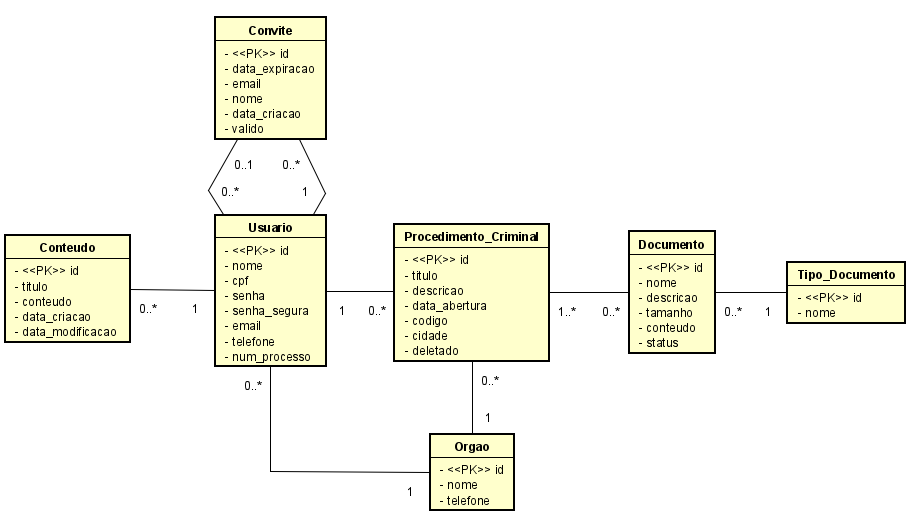
\includegraphics[width=1\linewidth]{conteudo//2 - ages I//conteudo//figures/figura2-esquema-bd}
    Fonte: \textit{Wiki} do projeto
    \label{fig:db-init}
\end{figure}

\begin{figure}[H]
    \centering
    \small
    \caption{Esquema lógico final do banco de dados do projeto Vítimas de Crime}
    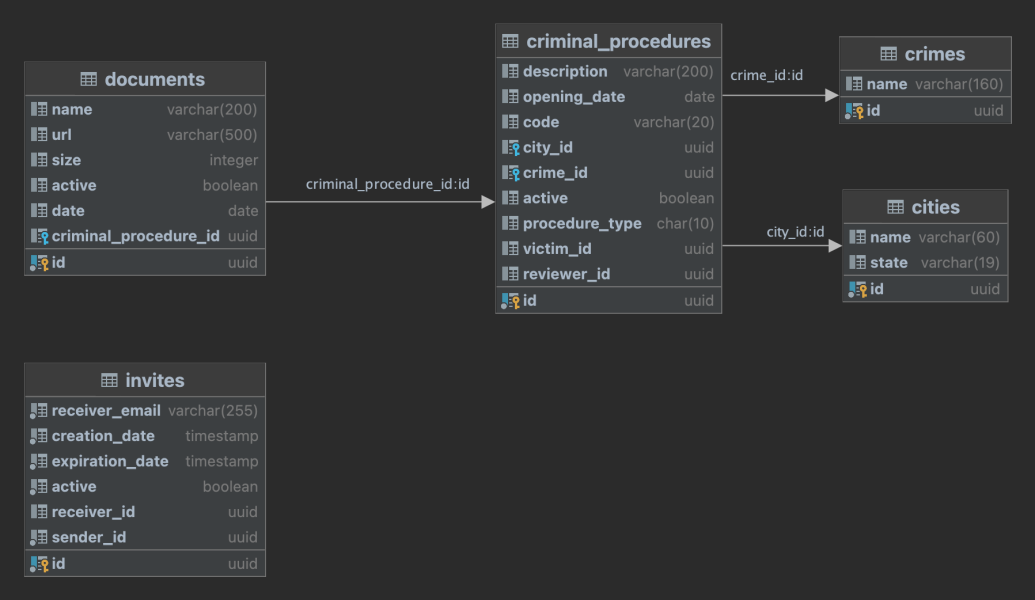
\includegraphics[width=1\linewidth]{conteudo//2 - ages I//conteudo//figures/figura3-logico-bd}
    Fonte: \textit{Wiki} do projeto
    \label{fig:db-schema}
\end{figure}

\subsection{Arquitetura Utilizada}
  A modelagem da arquitetura segue o design de cliente/servidor em camadas,
na qual os clientes requisitam serviços ou recursos e os servidores respondem,
fornecendo esses recursos, seguindo um paradigma de comunicação estabelecido. A
Figura 4 ilustra cada componente que representa o modelo idealizado.


\begin{figure}[H]
    \centering
    \small
    \caption{Diagrama dos componentes da arquitetura do projeto Vítimas de Crime}
    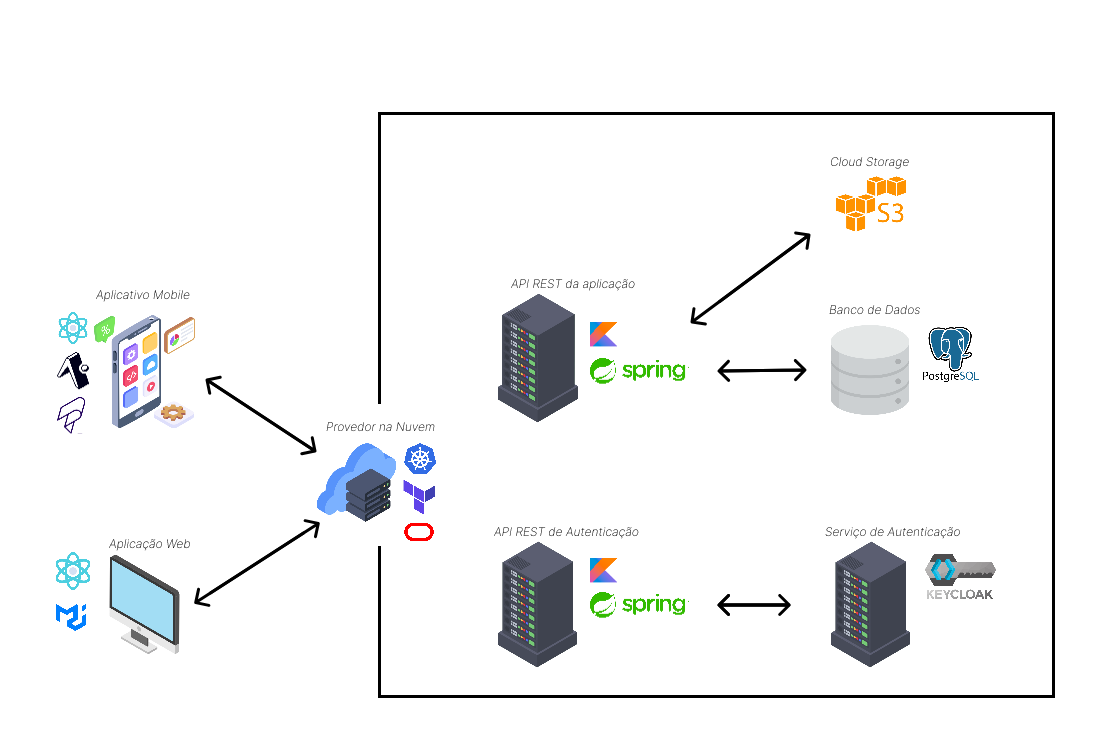
\includegraphics[width=1\linewidth]{conteudo//2 - ages I//conteudo//figures/figura4-diag-arq}
    Fonte: \textit{Wiki} do projeto
    \label{fig:components-arch}
\end{figure}

Na parte do servidor, as APIs REST da aplicação e de autenticação conversam
com seus respectivos recursos como o próprio banco de dados e o serviço de
autenticação. Os nossos clientes são os dispositivos mobile e web fazendo as
requisições a esse mesmo servidor.

\subsection{Protótipos das Telas Desenvolvidas}
  Os primeiros mockups do aplicativo mobile foram idealizados utilizando a
ferramenta Figma. Estes protótipos são apresentados nas Figuras 5, 6 e 7.

\begin{figure}[H]
    \centering
    \small
    \caption{Protótipo das telas mobile de cadastro do projeto Vítimas de Crime}
    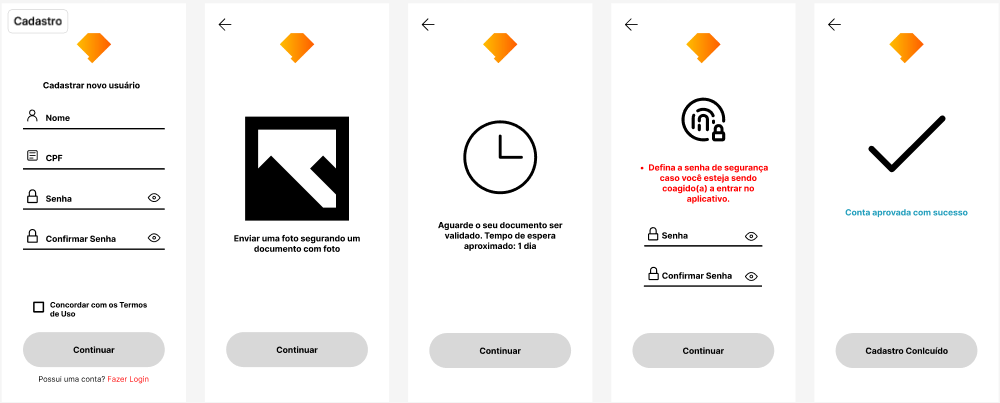
\includegraphics[width=1\linewidth]{conteudo//2 - ages I//conteudo//figures/figura5-prototipo-telas}
    Fonte: Figma do projeto
    \label{fig:mobile-signup}
\end{figure}

\begin{figure}[H]
    \centering
    \small
    \caption{Protótipo das telas mobile de envio de documentos do projeto Vítimas de Crime}
    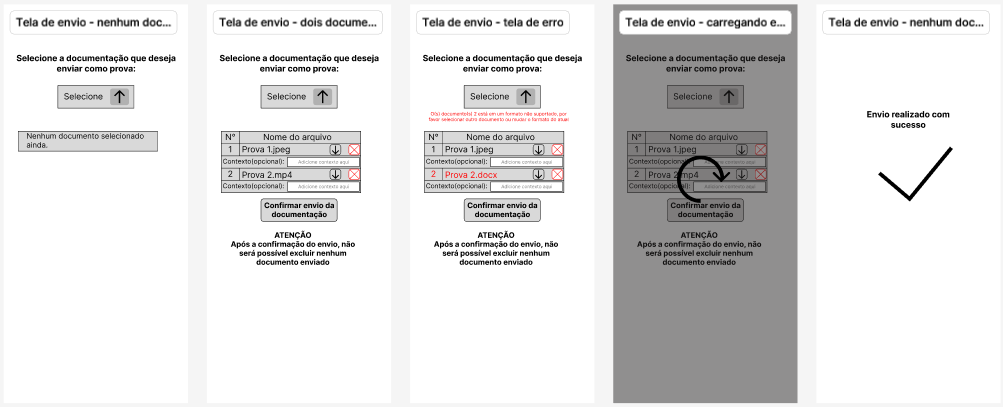
\includegraphics[width=1\linewidth]{conteudo//2 - ages I//conteudo//figures/figura6-prototipo-telas-resto}
    Fonte: Figma do projeto
    \label{fig:mobile-docs}
\end{figure}

\begin{figure}[H]
    \centering
    \small
    \caption{Protótipo das telas mobile de visualização de documentos do projeto Vítimas de Crime}
    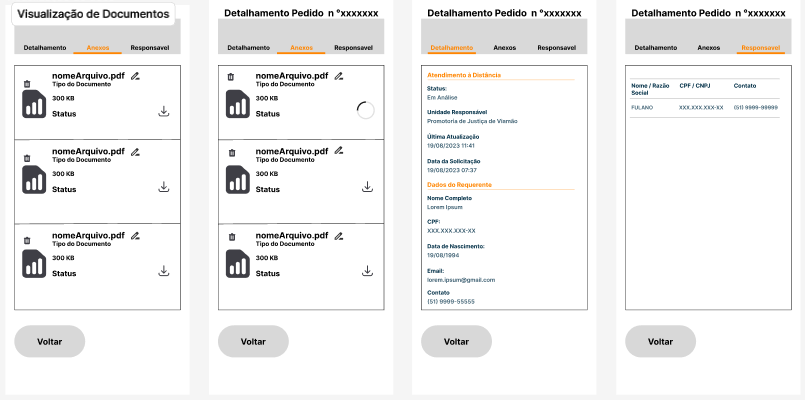
\includegraphics[width=1\linewidth]{conteudo//2 - ages I//conteudo//figures/figura7-resto-mais-mais-telas}
    Fonte: Figma do projeto
    \label{fig:mobile-visualization}
\end{figure}

Ao longo da implementação o projeto, realizou-se um style-guide a fim de
padronizar as telas e aprimorar a experiência do usuário. A Figura 8 apresenta
estas novas e últimas versões do aplicativo mobile.

\begin{figure}[H]
    \centering
    \small
    \caption{Telas finais mobile de boas-vidas, login, cadastro e home do projeto Vítimas de Crime}
    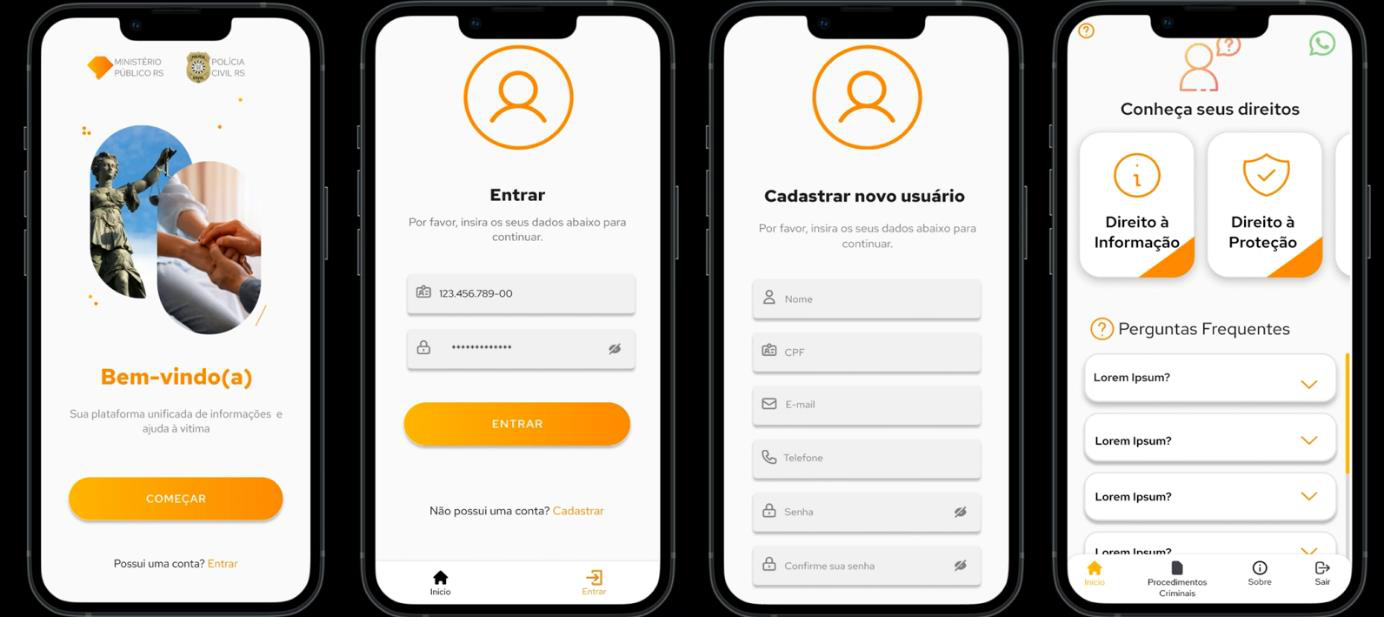
\includegraphics[width=1\linewidth]{conteudo//2 - ages I//conteudo//figures/figura8-telas-finais}
    Fonte: \textit{Wiki} do projeto
    \label{fig:final-mobile}
\end{figure}

Logo quando o aplicativo \textit{mobile} estava quase pronto, o time passou a desenvolver
as telas do \textit{website}. São apresentadas estas telas entregues nas Figuras 9 até 12.

\begin{figure}[H]
    \centering
    \small
    \caption{Tela web de boas-vidas do projeto Vítimas de Crime}
    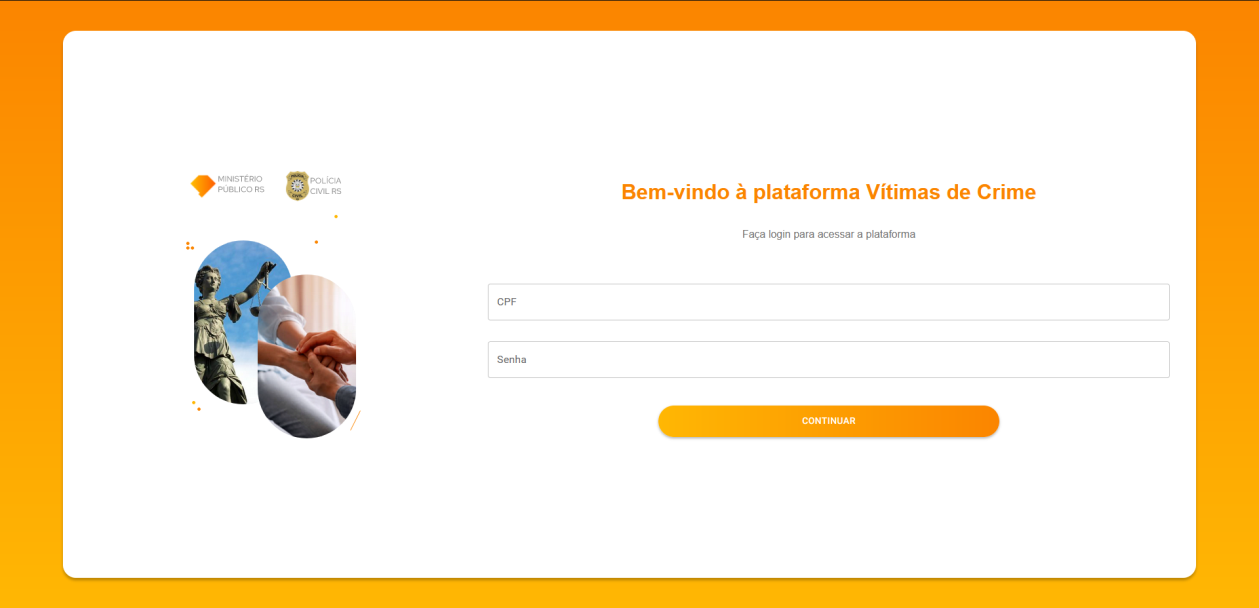
\includegraphics[width=1\linewidth]{conteudo//2 - ages I//conteudo//figures/figura9-web-tela-welcome}
    Fonte: Autor
    \label{fig:web-landing}
\end{figure}

\begin{figure}[H]
    \centering
    \small
    \caption{Tela web de procedimentos do projeto Vítimas de Crime}
    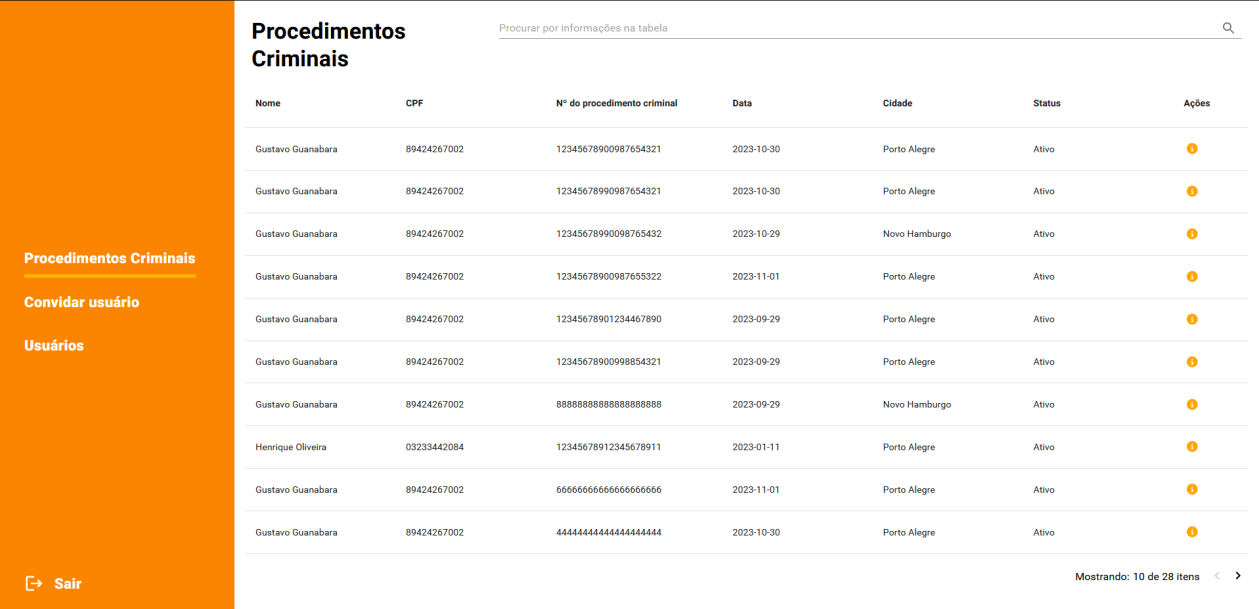
\includegraphics[width=1\linewidth]{conteudo//2 - ages I//conteudo//figures/figura10-web-tela-mais}
    Fonte: Autor
    \label{fig:web-procedures}
\end{figure}

\begin{figure}[H]
    \centering
    \small
    \caption{Tela web de convidar usuários do projeto Vítimas de Crime}
    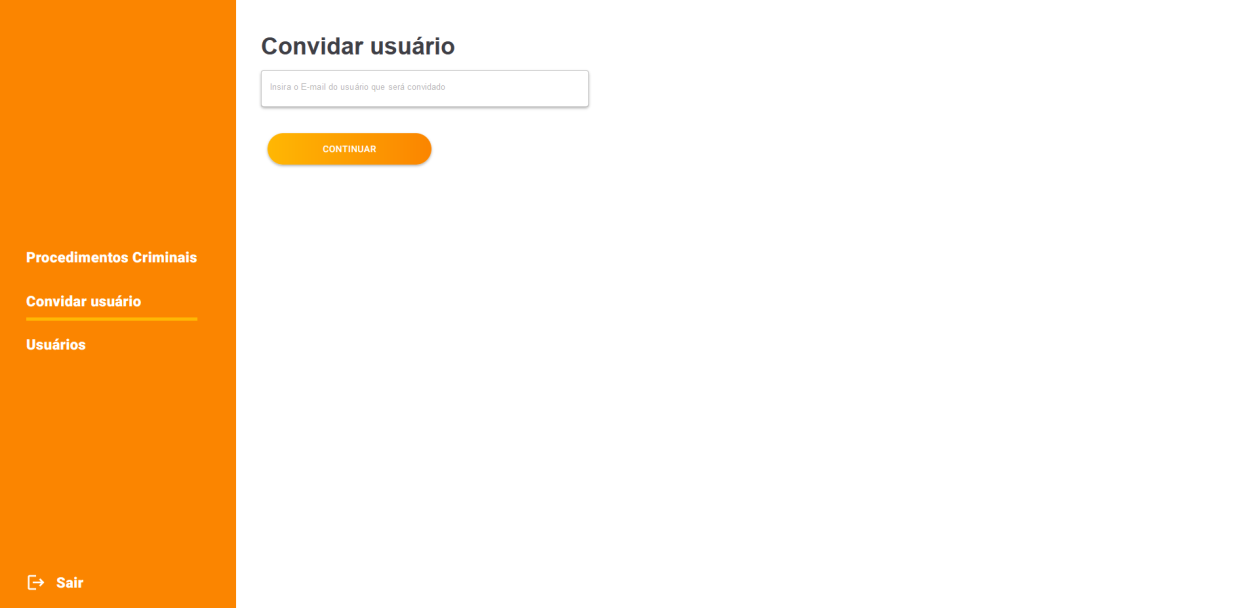
\includegraphics[width=1\linewidth]{conteudo//2 - ages I//conteudo//figures/figura11-tela-web-siuuu}
    Fonte: Autor
    \label{fig:web-invite}
\end{figure}

\begin{figure}[H]
    \centering
    \small
    \caption{Tela web de usuários do projeto Vítimas de Crime}
    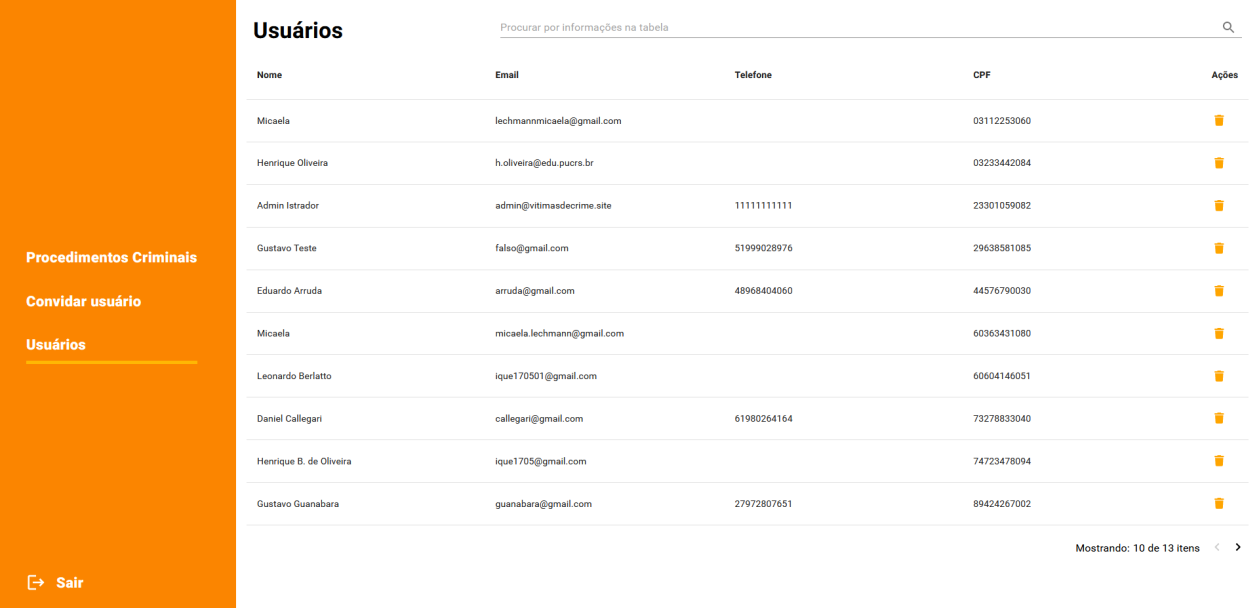
\includegraphics[width=1\linewidth]{conteudo//2 - ages I//conteudo//figures/figura12-tela-web-table}
    Fonte: Autor
    \label{fig:web-table}
\end{figure}

\subsection{Tecnologias Utilizadas}
  A implementação das APIs da aplicação e a gestão da autenticação no \textit{backend}
do projeto foram realizadas com a linguagem Kotlin, usando o framework Spring Boot,
Gradle como gerenciador de dependências e Selenium para testes de sistema. A
autenticação é gerenciada pela plataforma Keycloak, que implementa o protocolo
OAuth 2.

Além disso, foram utilizados recursos da AWS, incluindo S3 storage e EKS, e
para facilitar a configuração em diferentes ambientes e melhorar a escalabilidade
optamos pelo uso de containers Docker. Quanto ao \textit{frontend}, TypeScript foi escolhido
como a linguagem de principal, juntamente com React Native e Expo para o
desenvolvimento \textit{mobile}, enquanto React JS sendo utilizado para \textit{web}. \textit{Temp ref:
https://tools.ages.pucrs.br/vitimas-de-crime/wiki/-/wikis/Arquitetura do Projeto.}
